\section{Concurrent updates for Linux kernel}

\subsection{Case study:reverse mapping}

%$$$$$$$$$$$$$$$$$$$$$$$$$$$$$$$$$$$$$$$$$$$$$$$$$$$$$$$$$$$$$$$$$$$$$$$$$$$$$$$$
%Paragraph 1: Linux의 reverse mapping에 대한 자세한 설명 
%$$$$$$$$$$$$$$$$$$$$$$$$$$$$$$$$$$$$$$$$$$$$$$$$$$$$$$$$$$$$$$$$$$$$$$$$$$$$$$$$
리눅스 커널의 프로세스간 공유자원 중 하나인 reverse page mapping(rmap)은 fork가 수행될 때 update가 많이 발생하는
data structure이다.
Rmap의 anonymous page와 file page는 interval trees로 되어 있으며, 이것은 reverse page 성능
향상으로 위해 지속적으로 최적화가 ~\cite{CorbetLWNRMAP}~\cite{CorbetLWNANON}


따라서, fork를 병렬로 수행하면 reverse page mapping의 lock떄문에 scalability가 떨어진다.
Rmap의 anonymous page를 위한 rmap과 file mapped page을 위한 rmap 모두 문제가 있다. 


이번장은 LDU가 어떻게 리눅스에 적용되었는지에 대한 practial한 내용에 대해서 설명한다.

\subsection{anonymous page}

\begin{figure}[tb]
  \begin{center}
     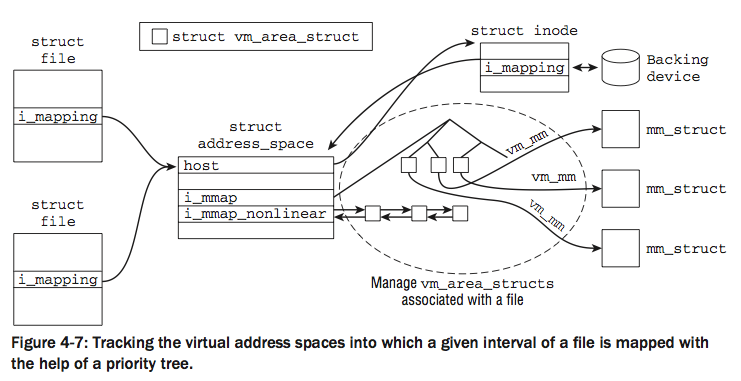
\includegraphics[width=0.5\textwidth,height=0.5\textheight,keepaspectratio]{fig/anon_vma_sample}
  \end{center}
  \caption{An example of applying the \deferu to file reverse mapping. }
  \label{fig:deferu2}
\end{figure}


%$$$$$$$$$$$$$$$$$$$$$$$$$$$$$$$$$$$$$$$$$$$$$$$$$$$$$$$$$$$$$$$$$$$$$$$$$$$$$$$$
%Paragraph 1: linux의 anon vma의 공유된 구조에 대한 설명
%$$$$$$$$$$$$$$$$$$$$$$$$$$$$$$$$$$$$$$$$$$$$$$$$$$$$$$$$$$$$$$$$$$$$$$$$$$$$$$$$
Anonymous rmap의 공유데이터는 서로 상당히 복잡하게 연결되어 있다.


%A page is said to be anonymous if it belongs to an anonymous memory region of a
%process (for instance, all pages in the User Mode heap or stack of a process
%are anonymous) Mapped page: a page is mapped to a file.
%For instance, all pages in the User Mode address spaces belonging to file
%memory mappings are mapped, as well as any other page included in the page
%cache.


\noindent
\textbf{GLDU.} 
%$$$$$$$$$$$$$$$$$$$$$$$$$$$$$$$$$$$$$$$$$$$$$$$$$$$$$$$$$$$$$$$$$$$$$$$$$$$$$$$$
%Paragraph 1: anon vma에 ldu 적용한 방법에 대한 설명 
%$$$$$$$$$$$$$$$$$$$$$$$$$$$$$$$$$$$$$$$$$$$$$$$$$$$$$$$$$$$$$$$$$$$$$$$$$$$$$$$$
Anonymous rmap을 위한 GLDU는 anon\_vma의 root structure에서 log를 저장하도록 하였다. 
anon rmap은 


\noindent
\textbf{PLDU.} 


%$$$$$$$$$$$$$$$$$$$$$$$$$$$$$$$$$$$$$$$$$$$$$$$$$$$$$$$$$$$$$$$$$$$$$$$$$$$$$$$$
%Paragraph 1: anon vma에 pldu를 적용이 힘든 이유 설명 
%$$$$$$$$$$$$$$$$$$$$$$$$$$$$$$$$$$$$$$$$$$$$$$$$$$$$$$$$$$$$$$$$$$$$$$$$$$$$$$$$
Anonymous page에는 per-core 방식을 적용하기 힘들다.
그 이유는 log를 저장하는 object가 너무 많은 object를 만들어서 global per-core hash table의 충돌이 너무 많이
발생하기 때문이다. 
이것은 또 다른 lock이 필요하므로 오히려 성능이 떨어진다. 
만약 per-core 방식을 적용하려면 하나의 per-core memory에 저장한 후 차후 log를 ojbect별 분리 하는 방법이 있으나, 
이 경우는  mix되어 있는 로그를 구별하면서 해당 data structure만 보호하는 lock을 사용하기가 어려우므로, global
lock을 사용해야한다.
결국 이 방법도 역시 global lock에 의한 scalability 문제가 있다.


\subsection{file mapped page}

\begin{figure}[tb]
  \begin{center}
     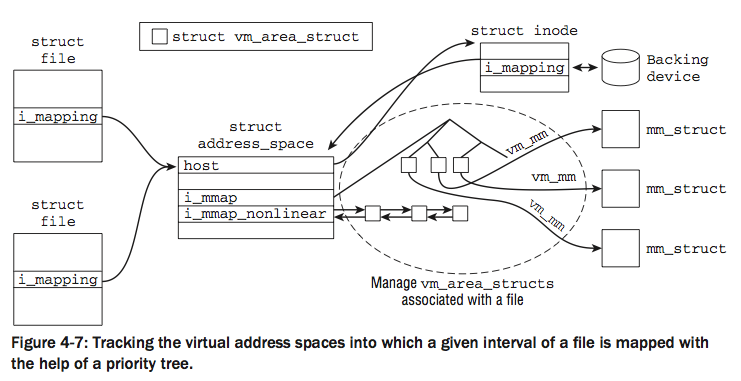
\includegraphics[width=0.5\textwidth,height=0.5\textheight,keepaspectratio]{fig/anon_vma_sample}
  \end{center}
  \caption{An example of applying the \deferu to file reverse mapping. }
  \label{fig:deferu}
\end{figure}
%$$$$$$$$$$$$$$$$$$$$$$$$$$$$$$$$$$$$$$$$$$$$$$$$$$$$$$$$$$$$$$$$$$$$$$$$$$$$$$$$
%Paragraph 1: linux의 file mapped page reverse mapping의 구조에 대한 설명
%$$$$$$$$$$$$$$$$$$$$$$$$$$$$$$$$$$$$$$$$$$$$$$$$$$$$$$$$$$$$$$$$$$$$$$$$$$$$$$$$
file rmap의 공유데이터는 anonymous rmap보다는 덜 복잡하게 연결되어 있다.
그림 x는 file rmap의 공유데이터를 보여준다. 



\noindent
\textbf{GLDU.} 
%$$$$$$$$$$$$$$$$$$$$$$$$$$$$$$$$$$$$$$$$$$$$$$$$$$$$$$$$$$$$$$$$$$$$$$$$$$$$$$$$
%Paragraph 1: file mapping에 ldu 적용한 방법에 대한 설명 
%$$$$$$$$$$$$$$$$$$$$$$$$$$$$$$$$$$$$$$$$$$$$$$$$$$$$$$$$$$$$$$$$$$$$$$$$$$$$$$$$
file mapping은 



\noindent
\textbf{PLDU.} 
%$$$$$$$$$$$$$$$$$$$$$$$$$$$$$$$$$$$$$$$$$$$$$$$$$$$$$$$$$$$$$$$$$$$$$$$$$$$$$$$$
%Paragraph 1: file mapping 에 pldu 적용한 방법에 대한 설명 
%$$$$$$$$$$$$$$$$$$$$$$$$$$$$$$$$$$$$$$$$$$$$$$$$$$$$$$$$$$$$$$$$$$$$$$$$$$$$$$$$
file mapping은 PLDU를 적용하는데 문제가 없다.
그 이유는 상대적으로 log의 header를 가지고 있는 address\_space가 상대적으로 적게 생성이 되어 hash 충돌이 적게 나타나기
때문에 scalability가 떨어지지 않는다.



%$$$$$$$$$$$$$$$$$$$$$$$$$$$$$$$$$$$$$$$$$$$$$$$$$$$$$$$$$$$$$$$$$$$$$$$$$$$$$$$$
%$$$$$$$$$$$$$$$$$$$$$$$$$$$$$$$$$$$$$$$$$$$$$$$$$$$$$$$$$$$$$$$$$$$$$$$$$$$$$$$$
%Reference Sentence 1
%$$$$$$$$$$$$$$$$$$$$$$$$$$$$$$$$$$$$$$$$$$$$$$$$$$$$$$$$$$$$$$$$$$$$$$$$$$$$$$$$




%$$$$$$$$$$$$$$$$$$$$$$$$$$$$$$$$$$$$$$$$$$$$$$$$$$$$$$$$$$$$$$$$$$$$$$$$$$$$$$$$
%Reference Sentence 2:LDU paper
%$$$$$$$$$$$$$$$$$$$$$$$$$$$$$$$$$$$$$$$$$$$$$$$$$$$$$$$$$$$$$$$$$$$$$$$$$$$$$$$$


%Figure : AIM7 실험 결과
%\begin{figure}[tb]
%  \begin{center}
%    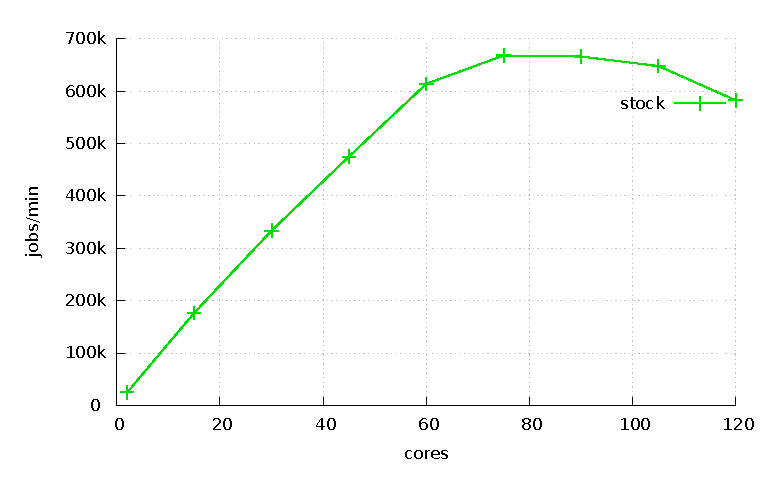
\includegraphics[scale=0.65]{graph/aim7_default.eps}
%  \end{center}
%  \caption{Scalability of AIM7 multiuser. This workload simultaneously create
%  many processes.
%  Up to 60 core, the stock Linux scale linearly, then they flattens out.}
%  \label{fig:aim7_default}
%\end{figure}
 
%In this section, we describe how to apply our concurrent update based on
%deferred update method to Linux.
%The Linux fork is associate with an anonymous page and a file page.
%When many processes are simultaneously created in Linux, 
%these two reverse mapping
%can become bottlenecks since their data structures are shared between
%processes.
%Figure~\ref{fig:aim7_default} shows the scalability problem in case
%of the fork-intensive workload that simultaneously creates many processes.
%Up to 60 core, the stock Linux scales linearly, then creating the reverse
%mapping becomes the bottleneck because their interval trees are protected by
%locks.
%Therefore, fork-intensive workload can pose a scalability bottleneck due to the
%update-heavy data
%structures~\cite{SilasBoydWickizerPth}~\cite{Andi2011adding}~\cite{Tim2013adding}.

%Figure mapped page에 대에 적용한  그림
%\begin{figure}[tb]
%%  \begin{center}
    %
    % \includegraphics[width=0.5\textwidth,height=0.5\textheight,keepaspectratio]{fig/deferu}
%  \end{center}
%  \caption{An example of applying the \deferu to file reverse mapping. }
%  \label{fig:deferu}
%\end{figure}


%Paragraph 6: DeferU 알고리즘 적용 - Mapped page - 리눅스 자료구조를 수정
%Figure~\ref{fig:deferu} gives an example of applying the \deferu to file
%reverse mapping and shows relationship between interval trees and lock-less
% lists.
%An interval tree contains two \code{virtual memory area}(\code{VMA}) nodes; 
%on the other hand, the lock-less list contains the right \code{VMA} as shown in
%Figure~\ref{fig:deferu}.
%It means that the right \code{VMA} has been deleted, and the synchronization
% has not been invoked. 

%In order to using the \deferu, the data structures involved in the
%head(\code{address\_space}) or the node(\code{vm\_area\_structure}) can be
% modified with \deferu's structure as shown in Figure~\ref{fig:deferu}. 
%In addition, programmer must replace \emph{physical update} with \emph{logical
%update} to eliminate the lock. 
%Before the corresponding readers need to be read, \deferu must call synchronize
%function to keep the consistency.
